\documentclass[
	a4paper,
	12pt,
	brazilian
]{article}

\usepackage[utf8]{inputenc}
\usepackage[T1]{fontenc}

\usepackage{amsmath, amsfonts, amssymb}
\usepackage{siunitx}

\usepackage[
top=2cm,
right=3cm,
bottom=2cm,
left=3cm
]{geometry}

\usepackage{xcolor}
\usepackage{tikz}
\usepackage{import}
\usepackage{float}

\usepackage{graphicx}
\usepackage{hyperref}
\usepackage{cleveref}
\usepackage{bm}
\usepackage{multirow}
\usepackage{cancel}
\usepackage[version=4]{mhchem}

\usepackage{config}

\begin{document}
	\section{Primeira questão}
	Calcular a pressão relativa no ponto indicado da tubulação. Resposta em \SI{}{\pascal} com uma casa decimal.\\\vspace{.5cm}
	
	\textbf{Dados:}
	\begin{itemize}
		\item Massa específica do fluido 1 = $\SI{13.1}{\gram/\centi\meter^{3}}$
		\item Massa específica do fluido 2 = $\SI{8.3}{\gram/\centi\meter^{3}}$
		\item Massa específica da água = $\SI{1000}{\kilogram/\meter^{3}}$
		\item $X=\SI{18.4}{\centi\meter}$
		\item $Y=\SI{8.3}{\centi\meter}$
		\item $Z=\SI{21.9}{\centi\meter}$
		\item $\beta=\SI{67.4}{\SIUnitSymbolDegree}$
	\end{itemize}
	\vspace{-8cm}
	\begin{flushright}
			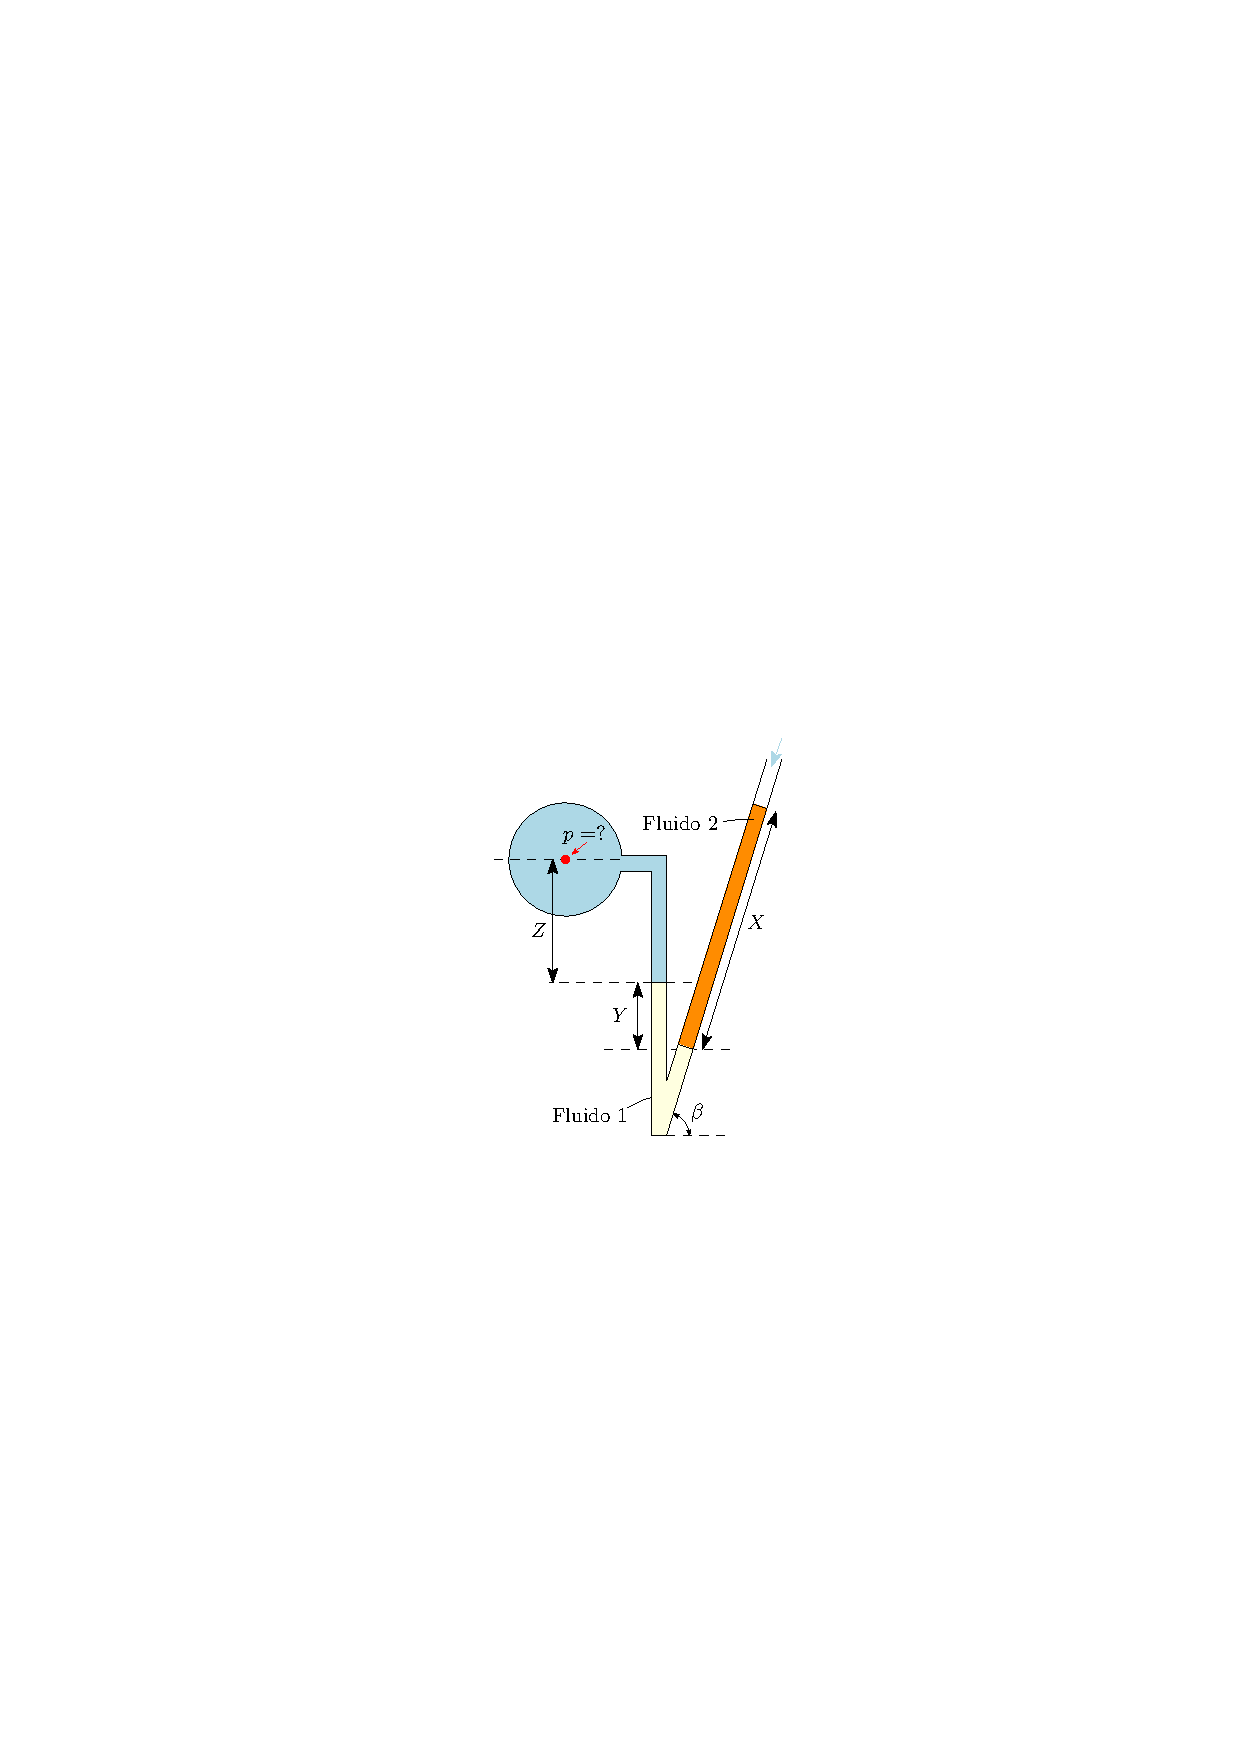
\includegraphics[width=0.4\linewidth]{assets/images/ex1}
	\end{flushright}
	\subsection{Solução}
	\begin{enumerate}
		\item[(1)] Estabelecer um referencial. É comum adotar a interface líquido-líquido mostrada.
		\begin{center}
			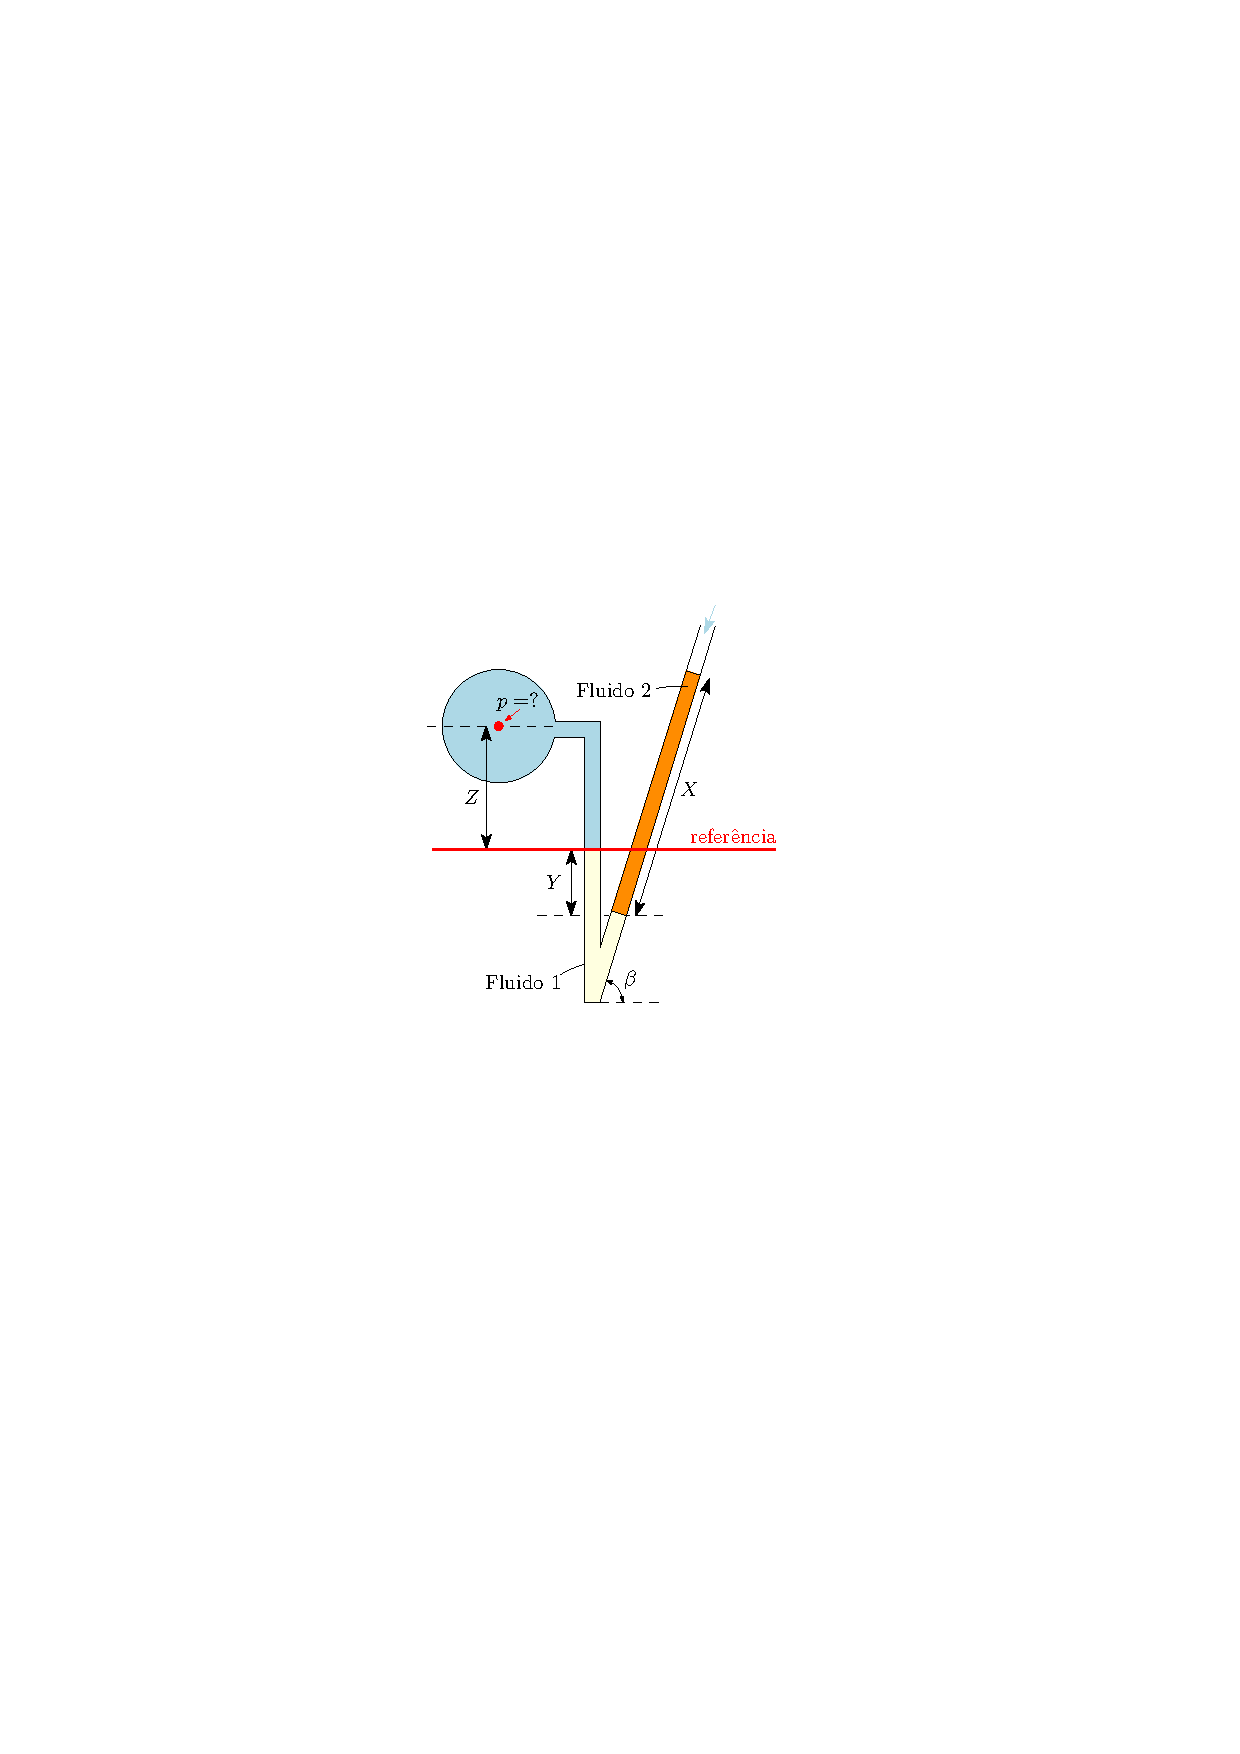
\includegraphics[width=.5\linewidth]{assets/images/referencia}
		\end{center}
		\item[(2)] Após estabelecer a cota de referência deve-se demarcar os pontos que serão analisados quanto a variação de pressão. Nesse caso, foram definidos dois pontos pertencentes à cota (1 e 2) e um ponto na superfície superior do fluido 2 (3) já que a pressão atmosférica na região simplifica os cálculos.
		\begin{center}
			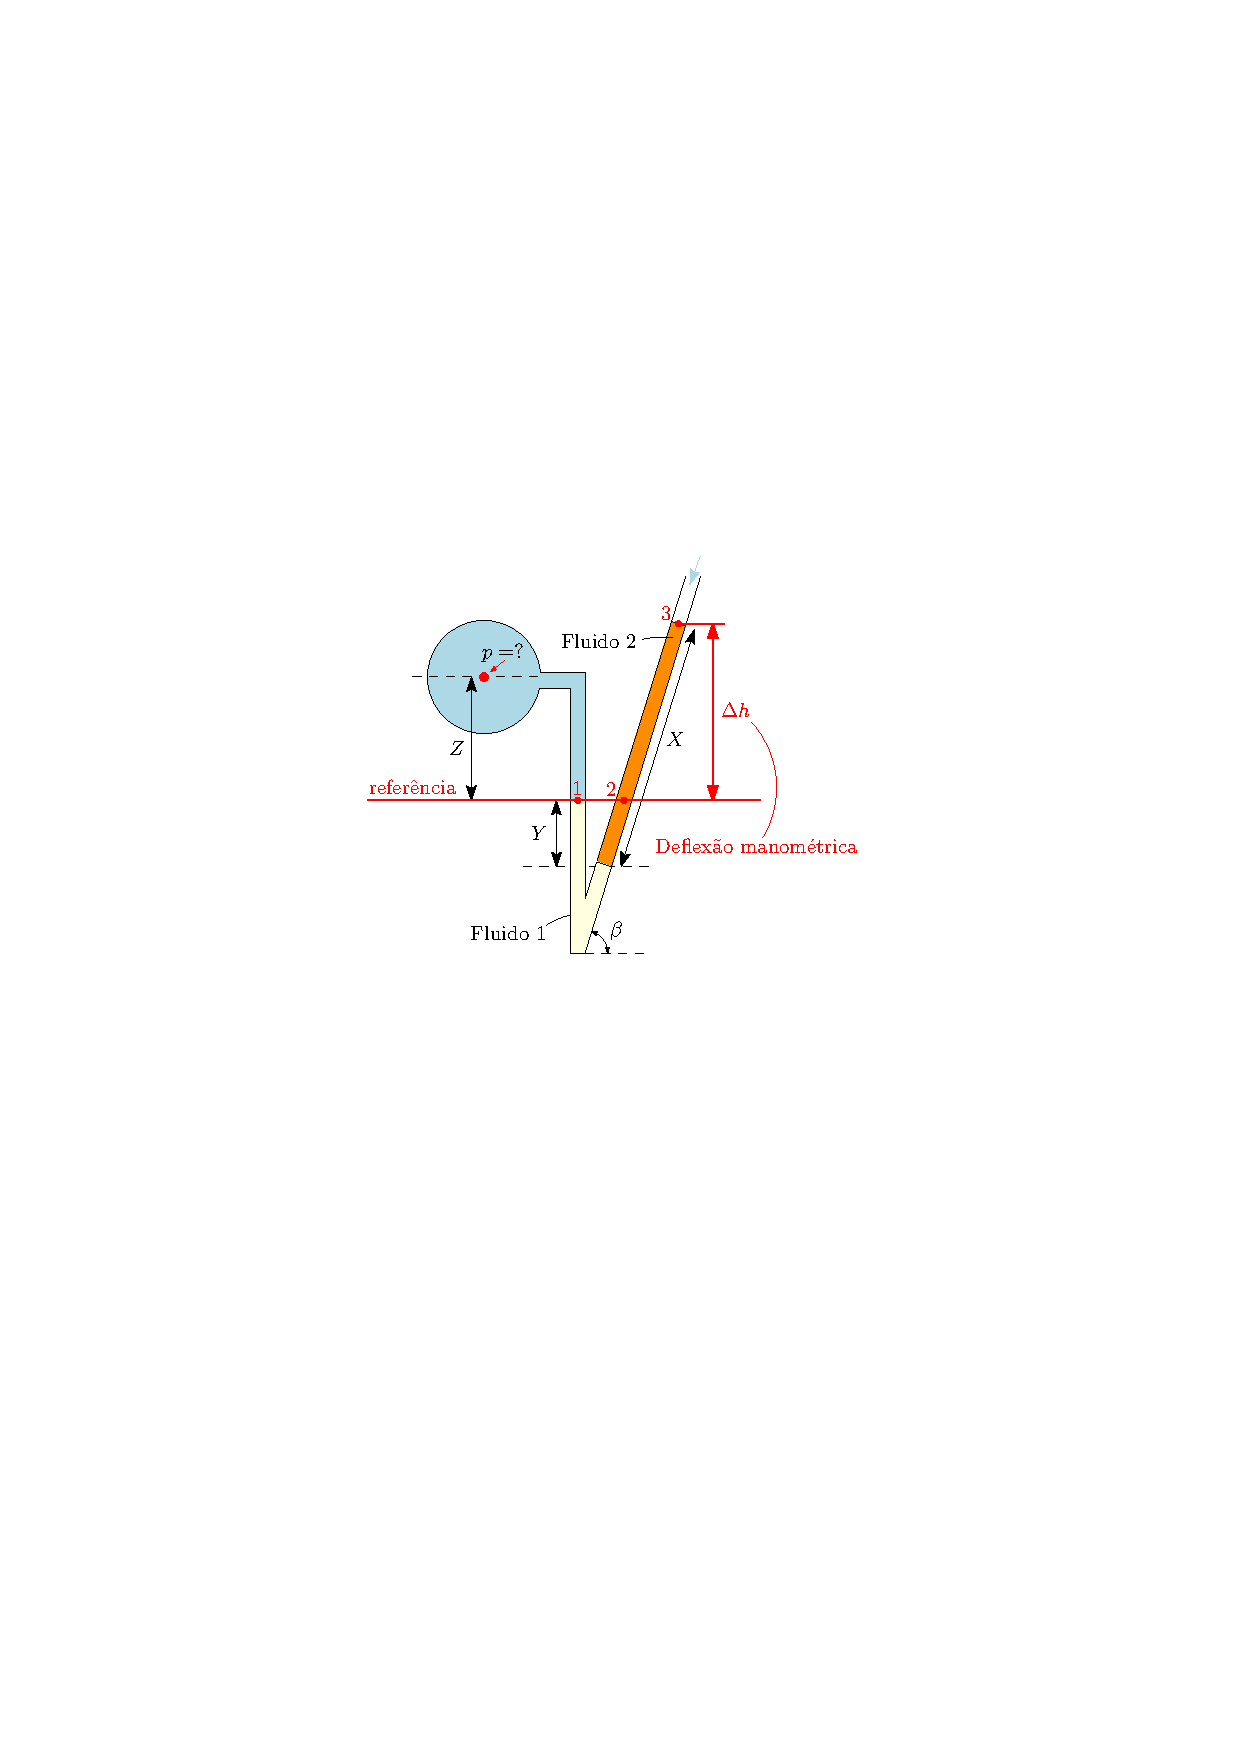
\includegraphics[width=.7\linewidth]{assets/images/pontos}
		\end{center}
		\item[(3)] Agora basta aplicar a lógica assimilada na parte de manômetros diferenciais e formular as equações para cada par de pontos como é visto abaixo
		$$
		\begin{cases}
			p_{1}-p_{4}=\gamma_{1}\cdot Y\\
			p_{4}-p=\gamma_{\ce{H2O}}\cdot Z
		\end{cases}
		$$
		Consequentemente
		\begin{equation}\label{eq1}
			p_{1}-p=\gamma_{1}\cdot Y+\gamma_{\ce{H2O}}\cdot Z
		\end{equation}
		\item[(4)] Aplicando os conceitos vistos em hidrostática, sabemos que pontos na mesma cota e \textbf{fluido} apresentam a mesma pressão (1 e 2), logo
		\begin{equation}
			p_{1}=p_{2}
		\end{equation}
		Ao analisar o tubo contendo o fluido 2
		\begin{equation}
			p_{2}-p_{3}=\gamma_{2}\cdot X\cdot\sin\beta
		\end{equation}
		Como p$_{3}=0$ e $p_{1}=p_{2}$
		\begin{equation}
			p_{1}=\gamma_{2}\cdot X\cdot\sin\beta
		\end{equation}
		Voltando em \eqref{eq1} e substituindo chegamos que
		\begin{equation}
			p=\gamma_{2}\cdot X\cdot\sin\beta-\gamma_{1}\cdot Y-\gamma_{\ce{H2O}}\cdot Z
		\end{equation}
		\item[(5)] Por fim, é necessário considerar as unidades no SI e converter as massas específicas dadas em gramas por centímetro cúbico ($\SI{}{\gram/\centi\meter^{3}}$) para quilogramas por metro cúbico ($\SI{}{\kilogram/\meter^{3}}$)
		\begin{eqnarray}
			\SI{}{\dfrac{\gram}{\centi\meter^{3}}}&=&\dfrac{10^{-3}}{(10^{-2})^{3}}\SI{}{\dfrac{\kilogram}{\meter^{3}}}\\
			&=&\dfrac{10^{-3}}{10^{-6}}\SI{}{\dfrac{\kilogram}{\meter^{3}}}\\
			&=&\SI{1000}{\dfrac{\kilogram}{\meter^{3}}}
		\end{eqnarray}
		\item[(6)] Ao multiplicar os valores de massa específica em gramas por centímetro cúbico por 1000 e substituir o restante dos valores de comprimento (em metros) na equação obtida para $p$
		\begin{eqnarray}
			p&=&8300\cdot 0.184\cdot\sin\SI{67.4}{\SIUnitSymbolDegree}-13\,100\cdot 0.083-1000\cdot 0.219\\
			&=&\SI{103.6}{\pascal}\approx\SI{0.1}{\kilo\pascal}
		\end{eqnarray}
	\end{enumerate}
	\section{Segunda questão}
	
	A figura abaixo ilustra um reservatório de água, cujo nível $h$ pode ser determinado utilizando um manômetro. Calcule o valor de $h$ em centímetros (\SI{}{\centi\meter}) com uma casa decimal.\\\vspace{.5cm}
	
	\textbf{Dados:}
	\begin{itemize}
		\item Reservatório contém água
		\item Manômetro contém líquido\\ manométrico: Mercúrio
		\item Peso específico da água:\\ $\gamma_{\ce{H2O}}=\SI{1000}{kgf/\meter^{3}}$
		\item Peso específico do mercúrio:\\ $\gamma_{\ce{Hg}}=\SI{13600}{kgf/\meter^{3}}$
		\item $x=\SI{29.2}{\centi\meter}$
		\item $y=\SI{10.9}{\centi\meter}$
	\end{itemize}
	\vspace{-7.5cm}
	\begin{flushright}
		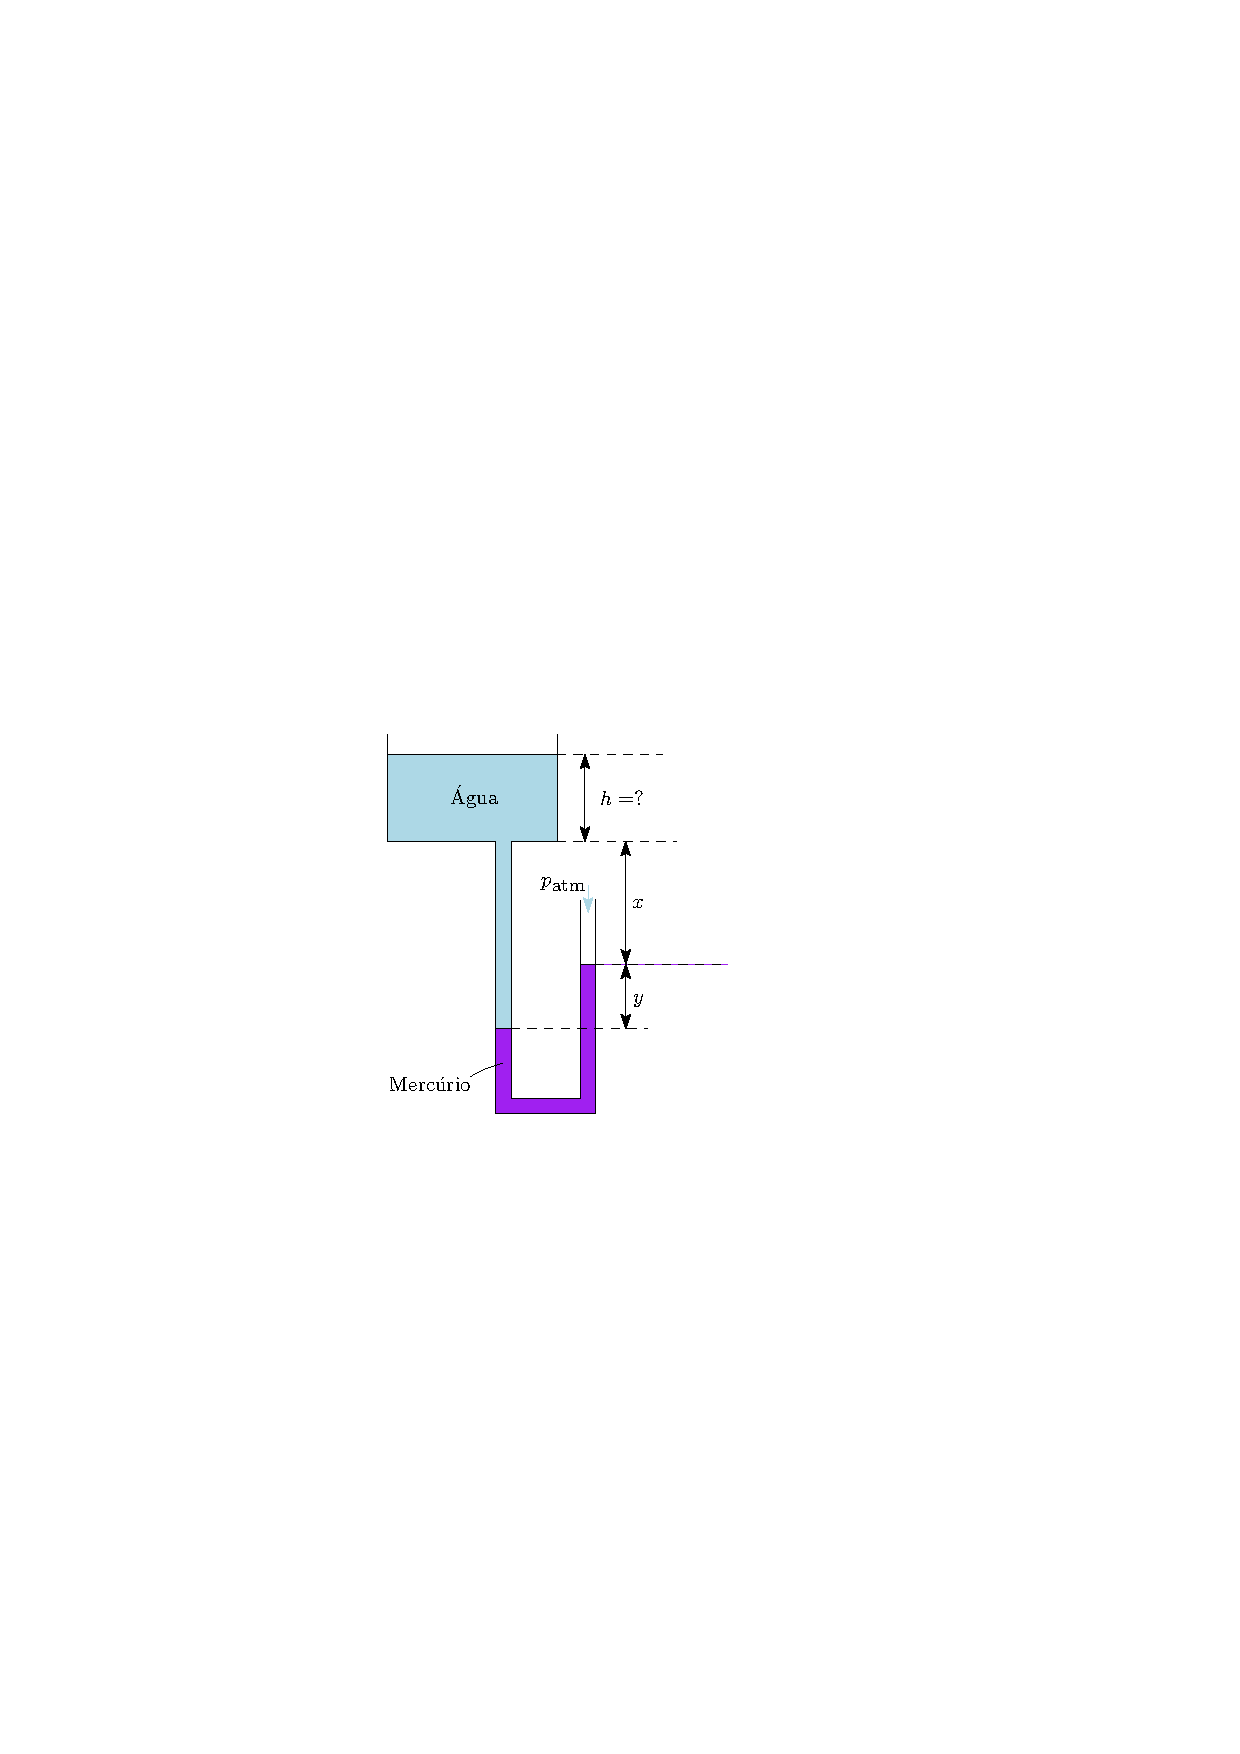
\includegraphics[width=.45\linewidth]{assets/images/ex2}
	\end{flushright}
	\begin{enumerate}
		\item[(1)] De maneira análoga a que foi usada na questão anterior, foi feito o estabelecimento de uma cota de referência e a marcação dos pontos para formular as equações
		\begin{center}
			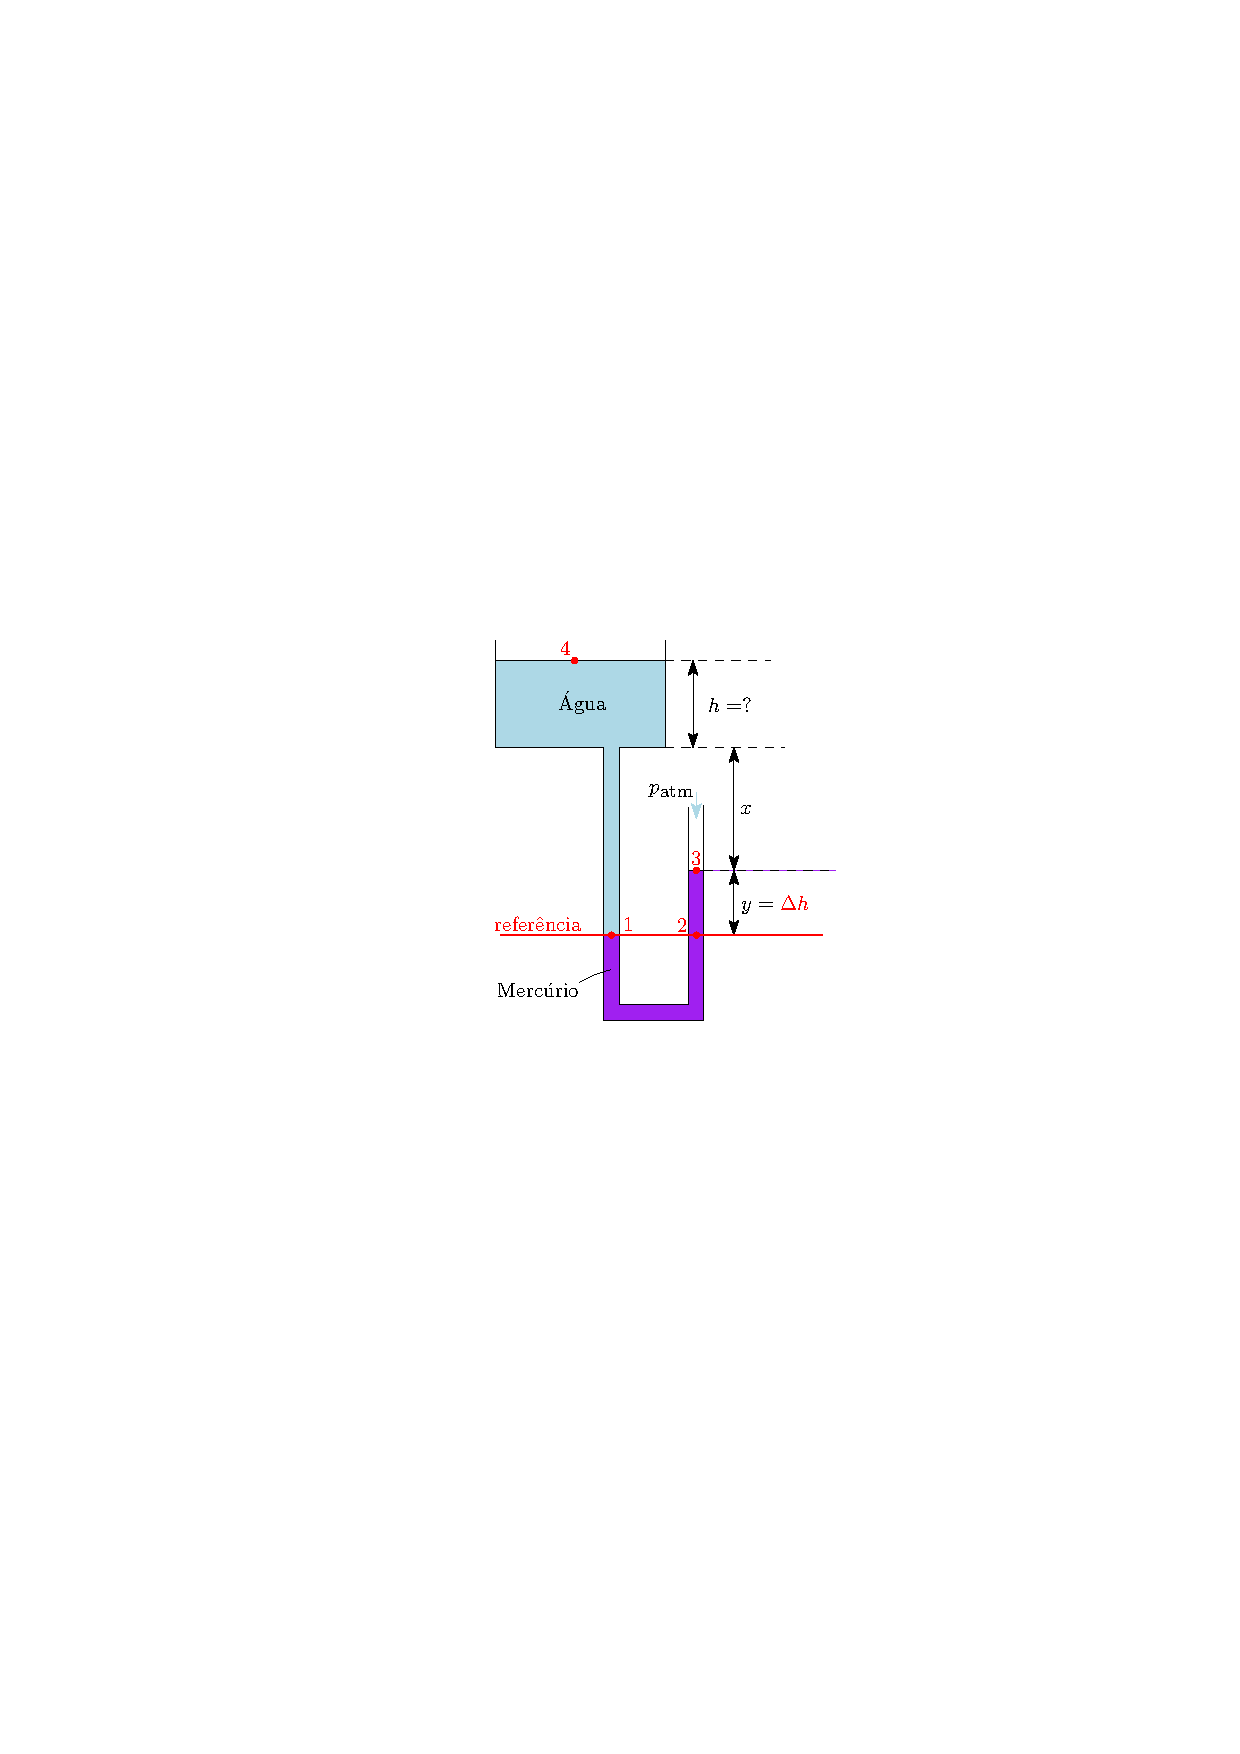
\includegraphics[width=.5\linewidth]{assets/images/referencia_2}
		\end{center}
		\item[(2)] As equações obtidas são
		$$
		\begin{cases}
			p_{1}-p_{4}=\gamma_{\ce{H2O}}\cdot (x+y+h)\\
			p_{2}-p_{3}=\gamma_{\ce{Hg}}\cdot y
		\end{cases}
		$$
		Assim
		\begin{eqnarray}
			p_{1}&=&p_{2}\\
			\gamma_{\ce{H2O}}\cdot (x+y+h)&=&\gamma_{\ce{Hg}}\cdot y\\
			h&=&\dfrac{(\gamma_{\ce{Hg}}-\gamma_{\ce{H2O}})\cdot y-\gamma_{\ce{H2O}}\cdot x}{\gamma_{\ce{H2O}}}
		\end{eqnarray}
	\end{enumerate}
	Considerando que 
	\begin{equation}
		\SI{1}{kgf}=\SI{9.81}{\newton}
	\end{equation}
	temos
	\begin{eqnarray}
		h&=&\dfrac{\cancel{9.81}\cdot (13600-1000)\cdot 10.9\cdot 10^{-2}-\cancel{9.81}\cdot 1000\cdot 29.2\cdot 10^{-2}}{\cancel{9.81}\cdot 1000}\\
		&=&\SI{1.0814}{\meter}\approx\SI{108.1}{\centi\meter}
	\end{eqnarray}
	\section{Terceira questão}
	Calcular a altura $h$ em \SI{}{\centi\meter} e apresentar o resultado com duas casas decimais.\\\vspace{.5cm}
	
	\textbf{Dados:}
	\begin{itemize}
		\item Pressão no ponto $A$:\\ 
		$p_{A}=\SI{148.67}{\kilo\pascal}$
		\item $X=\SI{59.4}{\centi\meter}$
		\item $Y=\SI{65.5}{\centi\meter}$
		\item Densidade do ar é desprezível.\\
		Pode-se assumir que a pressão\\
		é a mesma em todo o volume\\
		ocupado pelo ar.
		\item $\rho_{1}=\SI{1}{\gram/\centi\meter^{3}}$
		\item $\rho_{2}=\SI{13.6}{\gram/\centi\meter^{3}}$
		\item $\gamma_{4}=\SI{.13}{lbf/in^{3}}$
		\begin{itemize}
			\item $\SI{1}{lbf}=\SI{4.448}{\newton}$
			\item $\SI{1}{in}=\SI{25.4}{\milli\meter}$
			\item $g=\SI{9.81}{\meter/\second^{2}}$
		\end{itemize}
		\vspace{-11cm}
		\begin{flushright}
			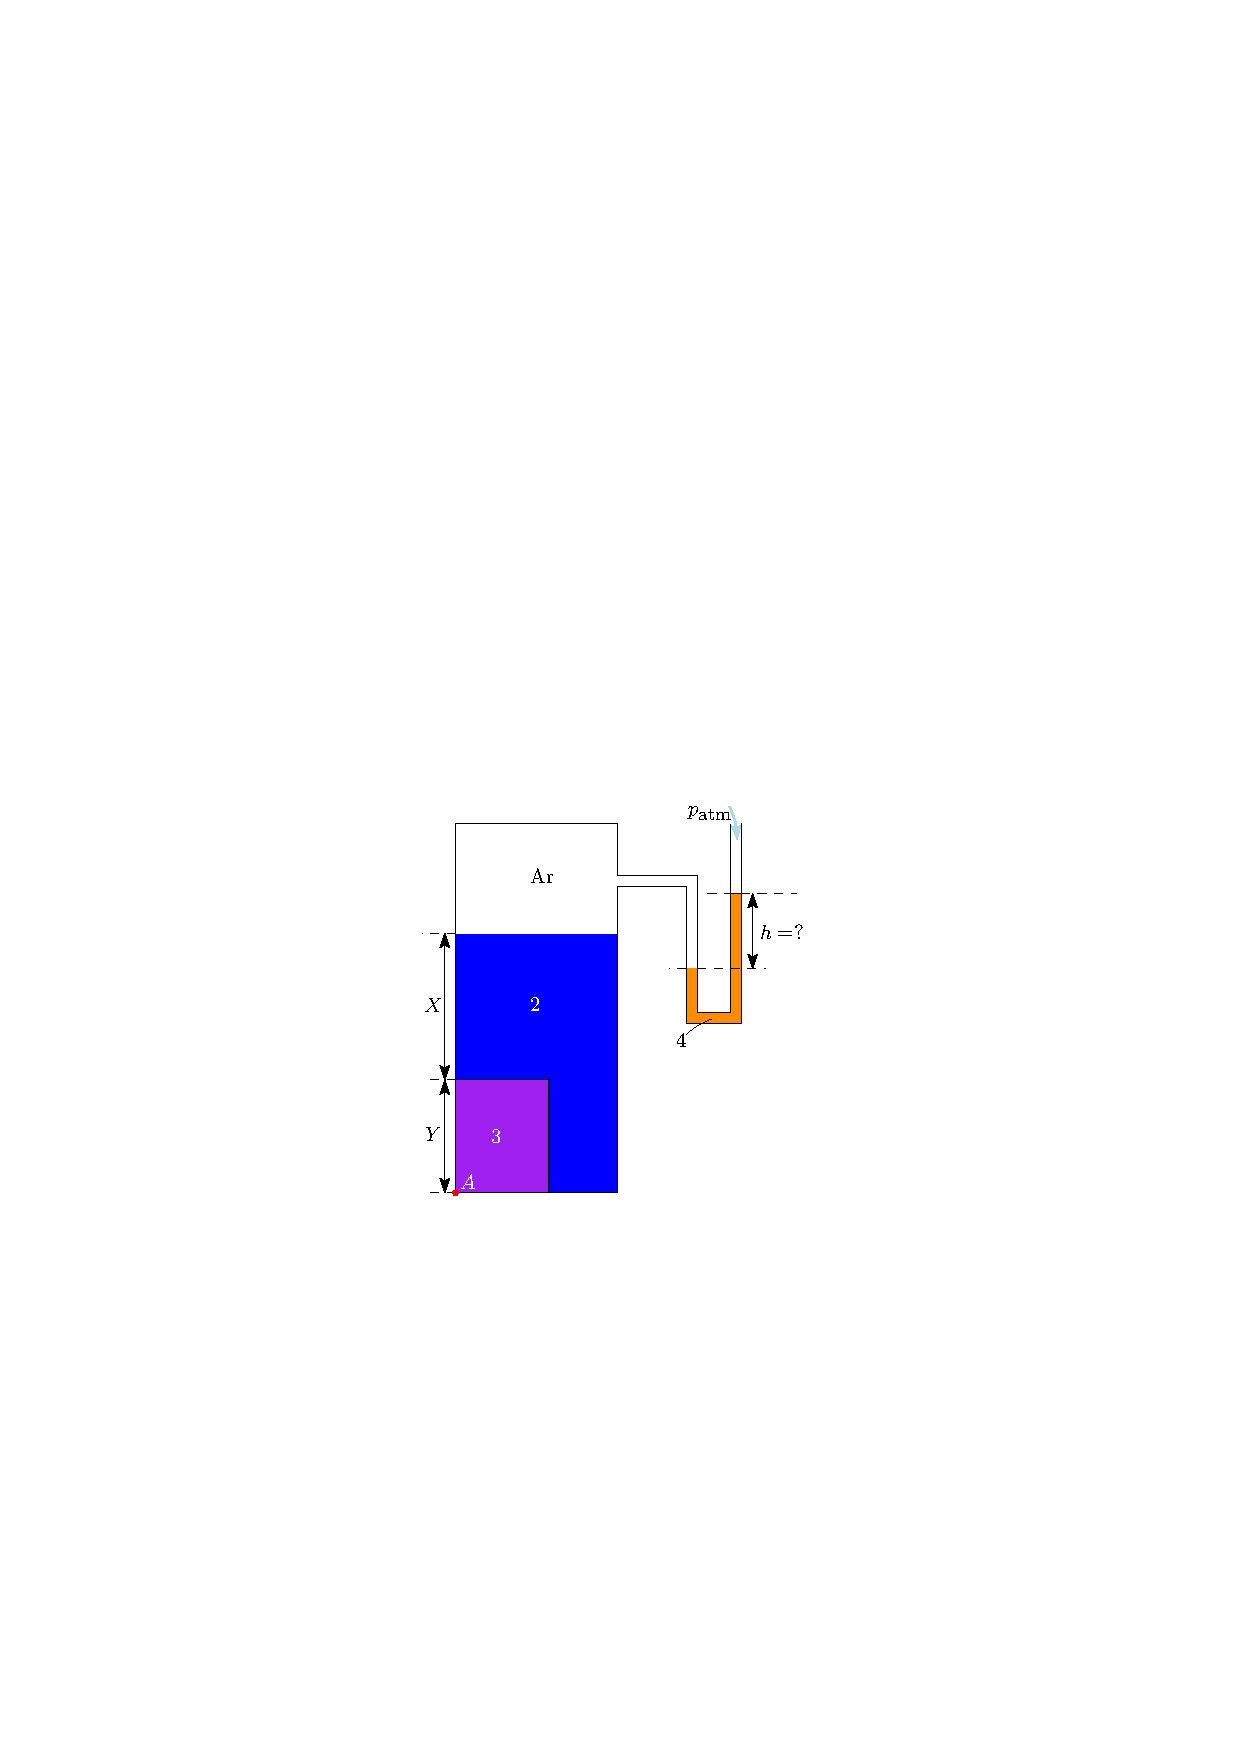
\includegraphics[width=.6\linewidth]{assets/images/ex3}
		\end{flushright}
	\end{itemize}
	\newpage
	\begin{enumerate}
		\item[(1)] Ao analisar o tubo contendo ar e o fluido 4, é preciso estabelecer o referencial igual ao que foi feito anteriormente, porém nesse exercício a pressão que o ar exerce no ponto 1 não é desprezível, tendo em vista que suas moléculas confinadas no volume, ao serem aproximadas (compressão), mantêm em equilíbrio o fluido presente no tubo. Para encontrar a equação que relaciona $X$, $Y$, $\gamma_{2}$, $\gamma_{3}$ podem ser utilizados alguns caminhos. A partir de um sistema de equações como é visto a seguir, temos\\
		
		eqs.$
		\begin{cases}
			p_{A}-p_{B}=\gamma_{3}\cdot Y\\
			p_{B}-p_{\textrm{Ar}}=\gamma_{2}\cdot X
		\end{cases}
		$\\\\\\
		\noindent Ao somar as duas equações\\
		
		$p_{A}-p_{\textrm{Ar}}=\gamma_{2}\cdot X+\gamma_{3}\cdot Y$
		
		$p_{\textrm{Ar}}=p_{A}-\gamma_{2}\cdot X-\gamma_{3}\cdot Y$
		\vspace{-4.5cm}
		\begin{flushright}
			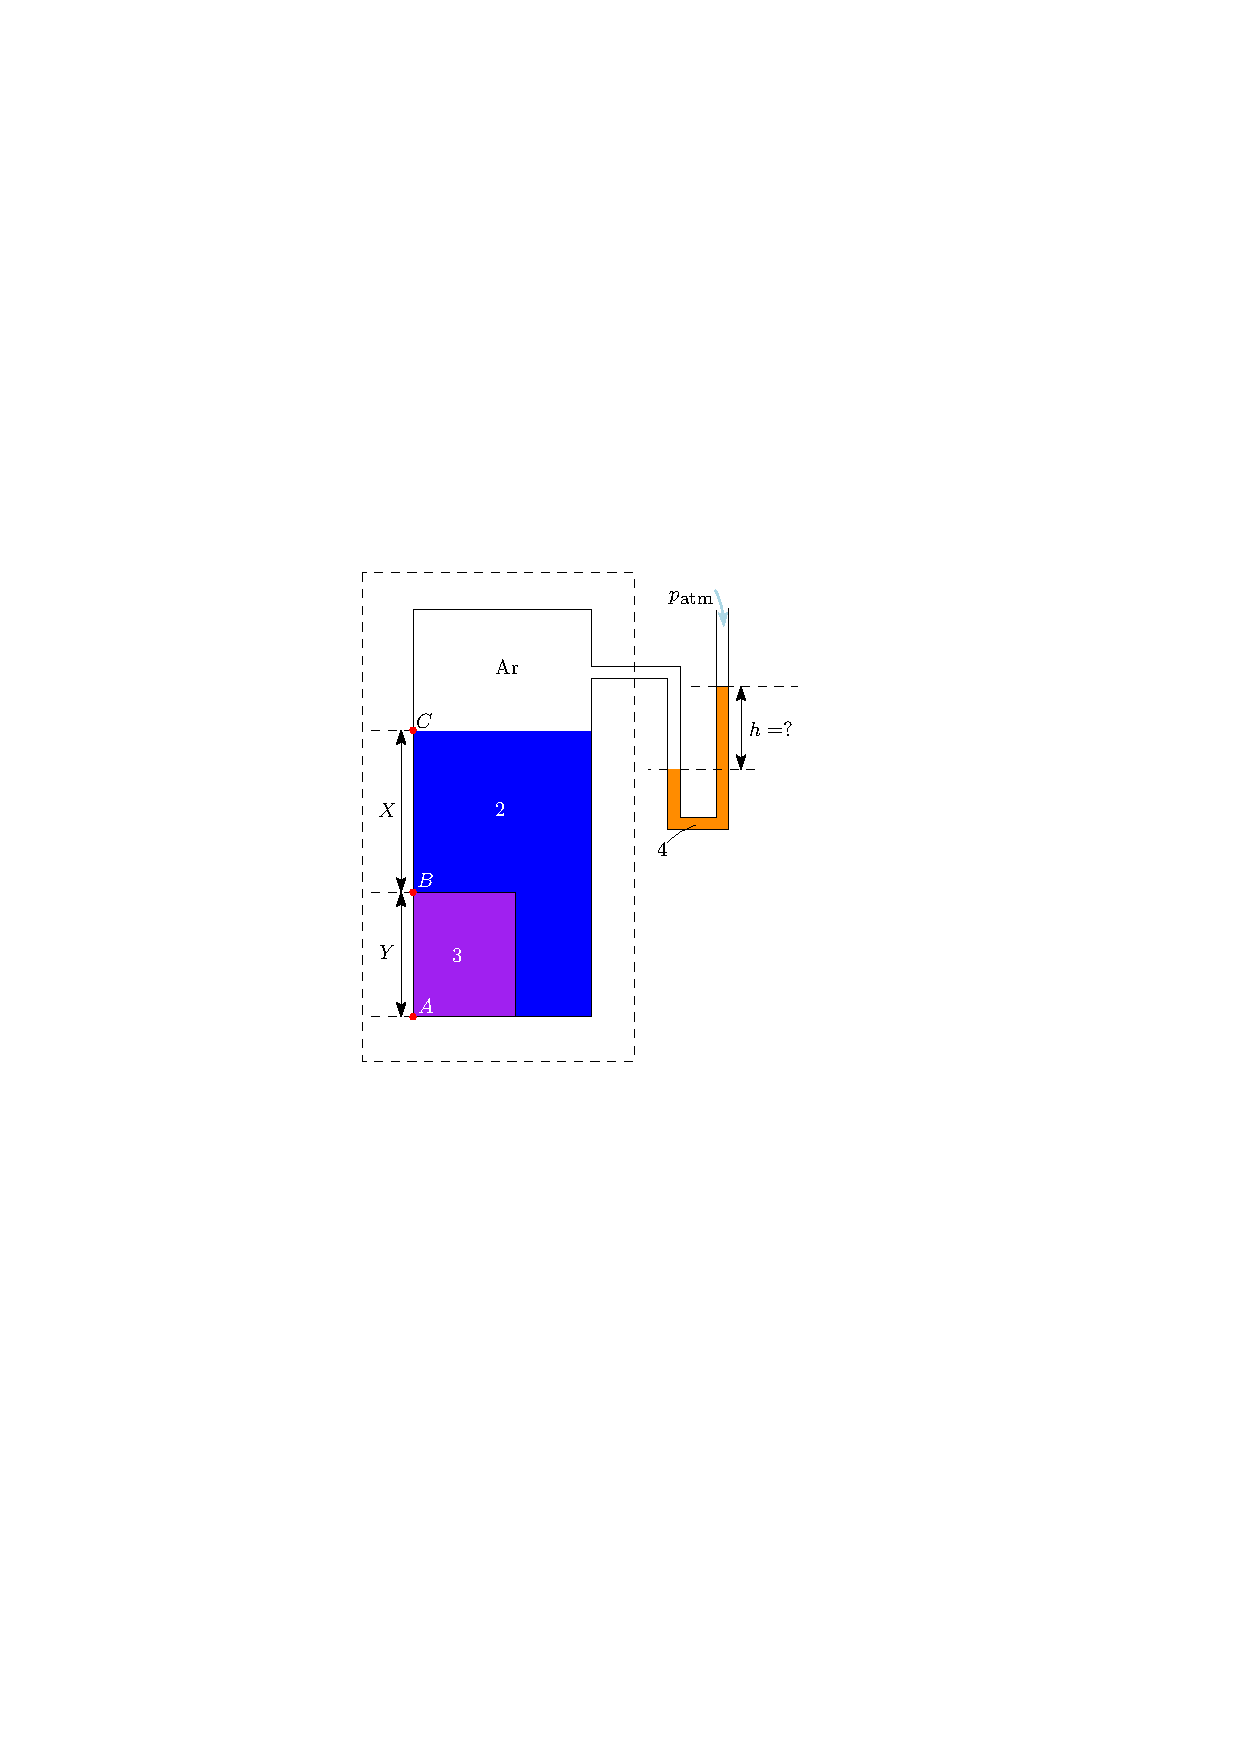
\includegraphics[width=.625\linewidth]{assets/images/pontos_3}
		\end{flushright}
		\item[(2)] Substituindo os dados do exercício conforme o SI, vem
		\begin{eqnarray}
			p_{\textrm{Ar}}&=&148\,670-1000\cdot 0.594-13600\cdot 0.655\\
			&=&\SI{139168}{\pascal}
		\end{eqnarray}
		\newpage
		\item[(3)] Após analisar o tubo com o fluido 4 e estabelecer o referencial visto abaixo, temos
		\begin{center}
			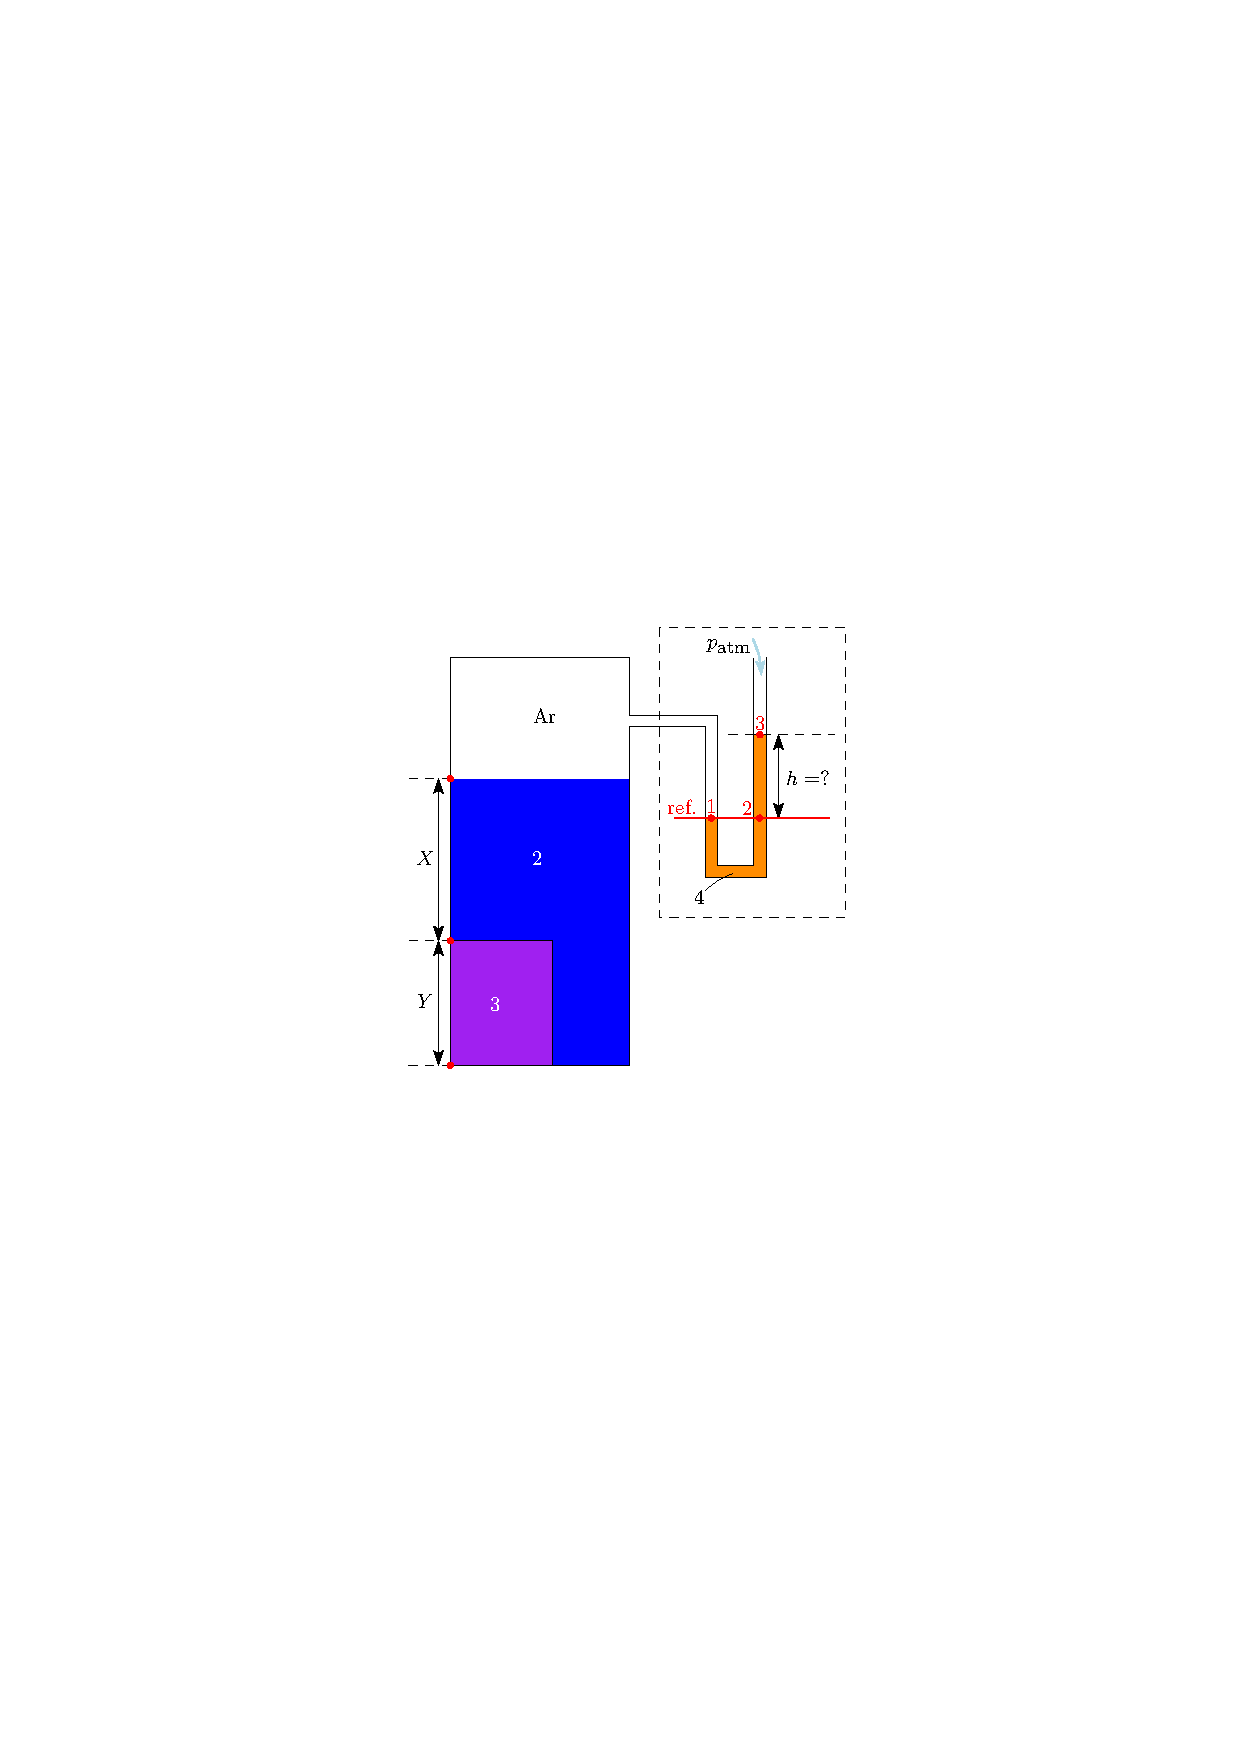
\includegraphics[width=.625\linewidth]{assets/images/pontos_3_1}
		\end{center}
		\begin{equation}
			p_{\textrm{Ar}}=p_{2}=p_{3}+\gamma_{4}\cdot h
		\end{equation}
		Como $p_{3}$ é desprezível
		\begin{equation}
			h=\dfrac{p_{\textrm{Ar}}}{\gamma_{4}}
		\end{equation}
		\item[(4)] Antes de substituir é preciso converter o peso específico fornecido em $\SI{}{lbf/in^{3}}$ para $\SI{}{\newton/\meter^{3}}$
		\begin{eqnarray}
			\gamma_{4}&=&\SI{0.13}{\dfrac{lbf}{in^{3}}}\\
			&=&\dfrac{0.13\cdot 4.448}{0.0254^{3}}\SI{}{\dfrac{\newton}{\meter^{3}}}\\
			&=&\SI{35286.3697853}{\dfrac{\newton}{\meter^{3}}}
		\end{eqnarray}
		\item[(5)] Assim
		\begin{equation}
			h=\SI{3.9439}{\meter}=\SI{394.39}{\centi\meter}
		\end{equation}
	\end{enumerate}
	\section{Quarta questão}
	Para a figura apresentada, calcular a pressão absoluta no final do tubo, onde há uma câmara contendo ar comprimido. Resposta em \SI{}{\kilo\pascal} com uma casa decimal.\\\vspace{.5cm}
	
	\textbf{Dados:}
	\begin{itemize}
		\item $a=\SI{4}{in}$
		\item $b=\SI{16.4}{in}$
		\item $\beta=\SI{72.7}{\SIUnitSymbolDegree}$
		\item $d_{l}=9.5$
		\item $p_{\textrm{atm}}=\SI{101325}{\newton/\meter^{2}}$
		\item $\SI{1}{in}=\SI{2.54}{\centi\meter}$
		\item $\rho_{\ce{H2O}}=\SI{1000}{\kilogram/\meter^{3}}$ (substância padrão)
		\item $g=\SI{9.81}{\meter/\second^{2}}$
		\item Dica: A massa específica do ar é desprezível e pode-se assumir que a pressão é a mesma em todo o volume ocupado por ar comprimido.
	\end{itemize}
	\begin{center}
		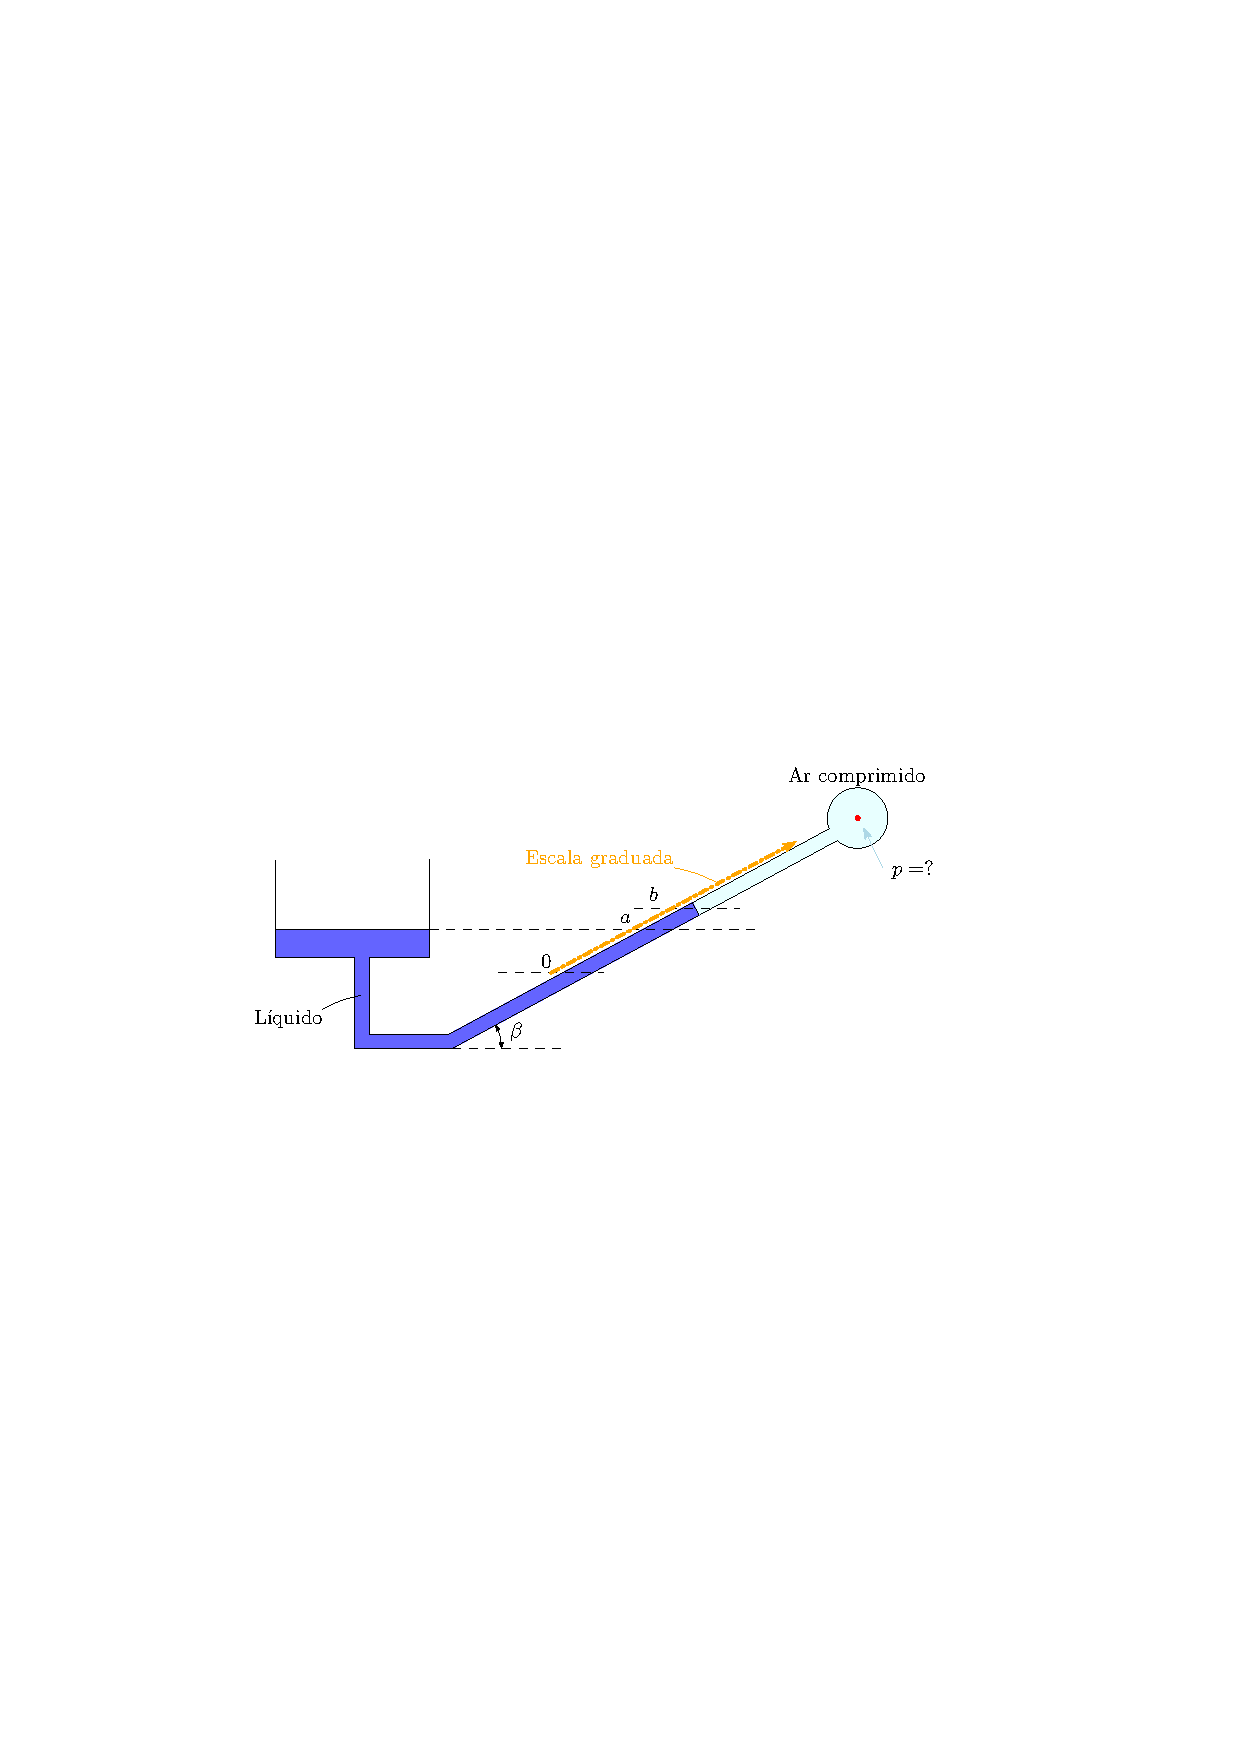
\includegraphics[width=1\linewidth]{assets/images/ex4}
	\end{center}
	Após marcar o ponto 1 e considerar que ele está sujeito à pressão atmosférica, adotando o referencial apresentado abaixo é possível escrever
	\begin{center}
		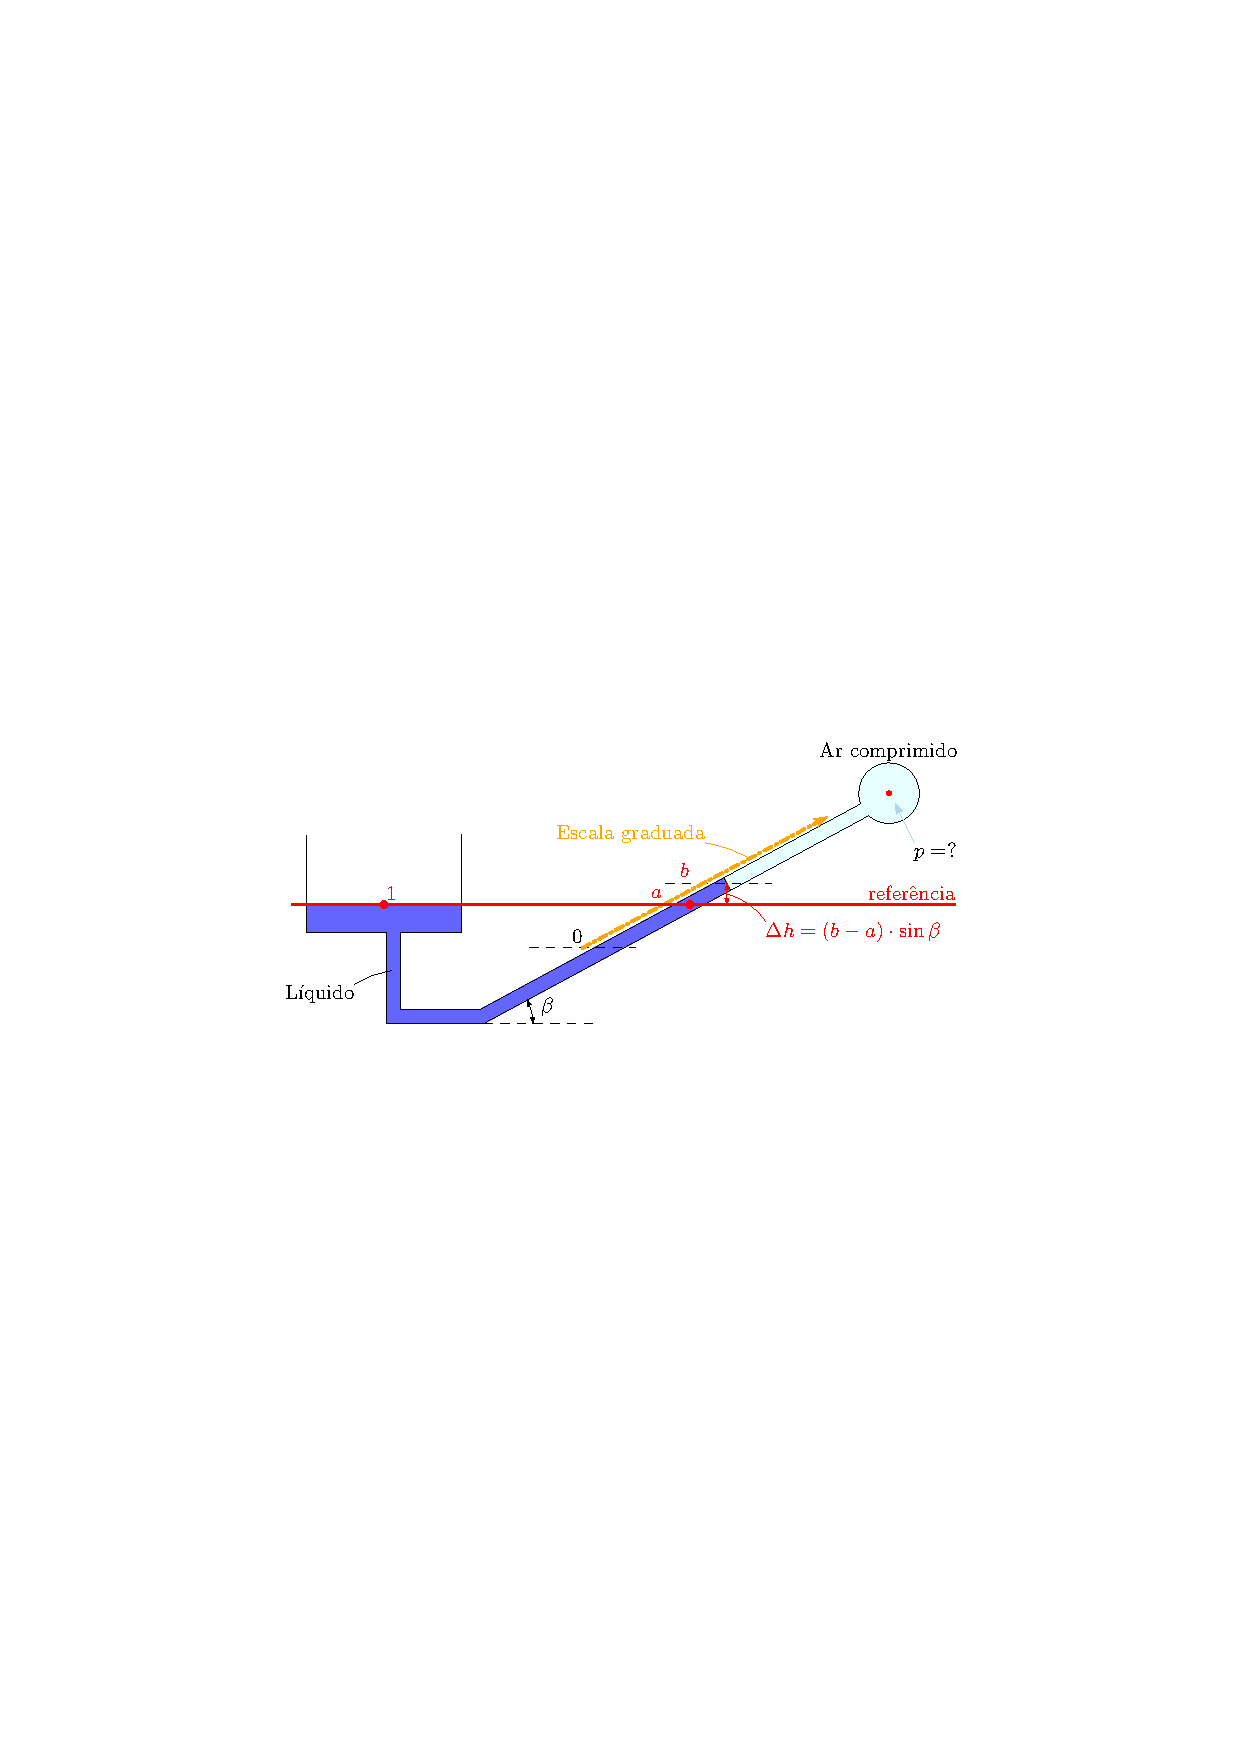
\includegraphics[width=1\linewidth]{assets/images/referencia_4}
	\end{center}
	\begin{equation}
		p_{1}=p_{\textrm{atm}}=p_{a}
	\end{equation}
	Fazendo $p_{a}-p_{b}$ temos
	\begin{eqnarray}
		p_{a}-p_{b}&=&\gamma_{l}\cdot\Delta h\\
		&=&\gamma_{l}\cdot (b-a)\cdot\sin\beta\\
		&=&\rho_{l}\cdot g\cdot (b-a)\cdot\sin\beta\\
		&=&9500\cdot 9.81\cdot (16.4-4)\cdot 0.0254\cdot\sin\SI{72.7}{\SIUnitSymbolDegree}\\
		&=&\SI{28024.8046462}{\pascal}
	\end{eqnarray}
	Como $p_{1}=p_{a}$ podemos escrever
	\begin{eqnarray}
		101\,325-p_{b}&=&28\,024.804\,646\,2\\
		p_{b}&=&\SI{73\,300.1953538}{\pascal}\\
		p_{b}&=&p=\SI{73.3}{\kilo\pascal}
	\end{eqnarray}
	Como a pressão absoluta é dada pela soma da pressão relativa (no ponto) e a pressão atmosférica, temos 
	\begin{eqnarray}
		(p_{\textrm{abs}})_{b}&=&p_{\textrm{atm}}+\overbrace{p_{b}}^{\textrm{relativa}}\\
		&=&101.325+73.3\approx\SI{174.6}{\kilo\pascal}
	\end{eqnarray}
	\section{Quinta questão}
	Calcule a pressão relativa indicada pelo manovacuômetro para a situação ilustrada abaixo. Resposta em \SI{}{\milli\bar} (milibar) com uma casa decimal. Caso a pressão seja negativa, o resultado deve conter o sinal negativo.\vspace{.5cm}
	
	\textbf{Dados:}
	\begin{enumerate}
		\item Densidade dos fluidos indicados no desenho:
		\begin{itemize}
			\item $d_{A}=2.3$
			\item $d_{B}=5.4$
			\item $d_{C}=1.3$
			\item $d_{D}=6.9$
		\end{itemize}
		\item Comprimento em polegadas ('')
		\item $\SI{1}{in}=\SI{2.53}{\centi\meter}$
		\item Massa específica da água (substância padrão):\\
		$\rho_{\ce{H2O}}=\SI{1000}{\kilogram/\meter^{3}}$
		\item $g=\SI{9.81}{\meter/\second^{2}}$
		\item A massa específica do ar é desprezível e pode-se assumir que a pressão é a mesma em todo o volume do tanque ocupado por ar.
	\end{enumerate}
	\begin{center}
		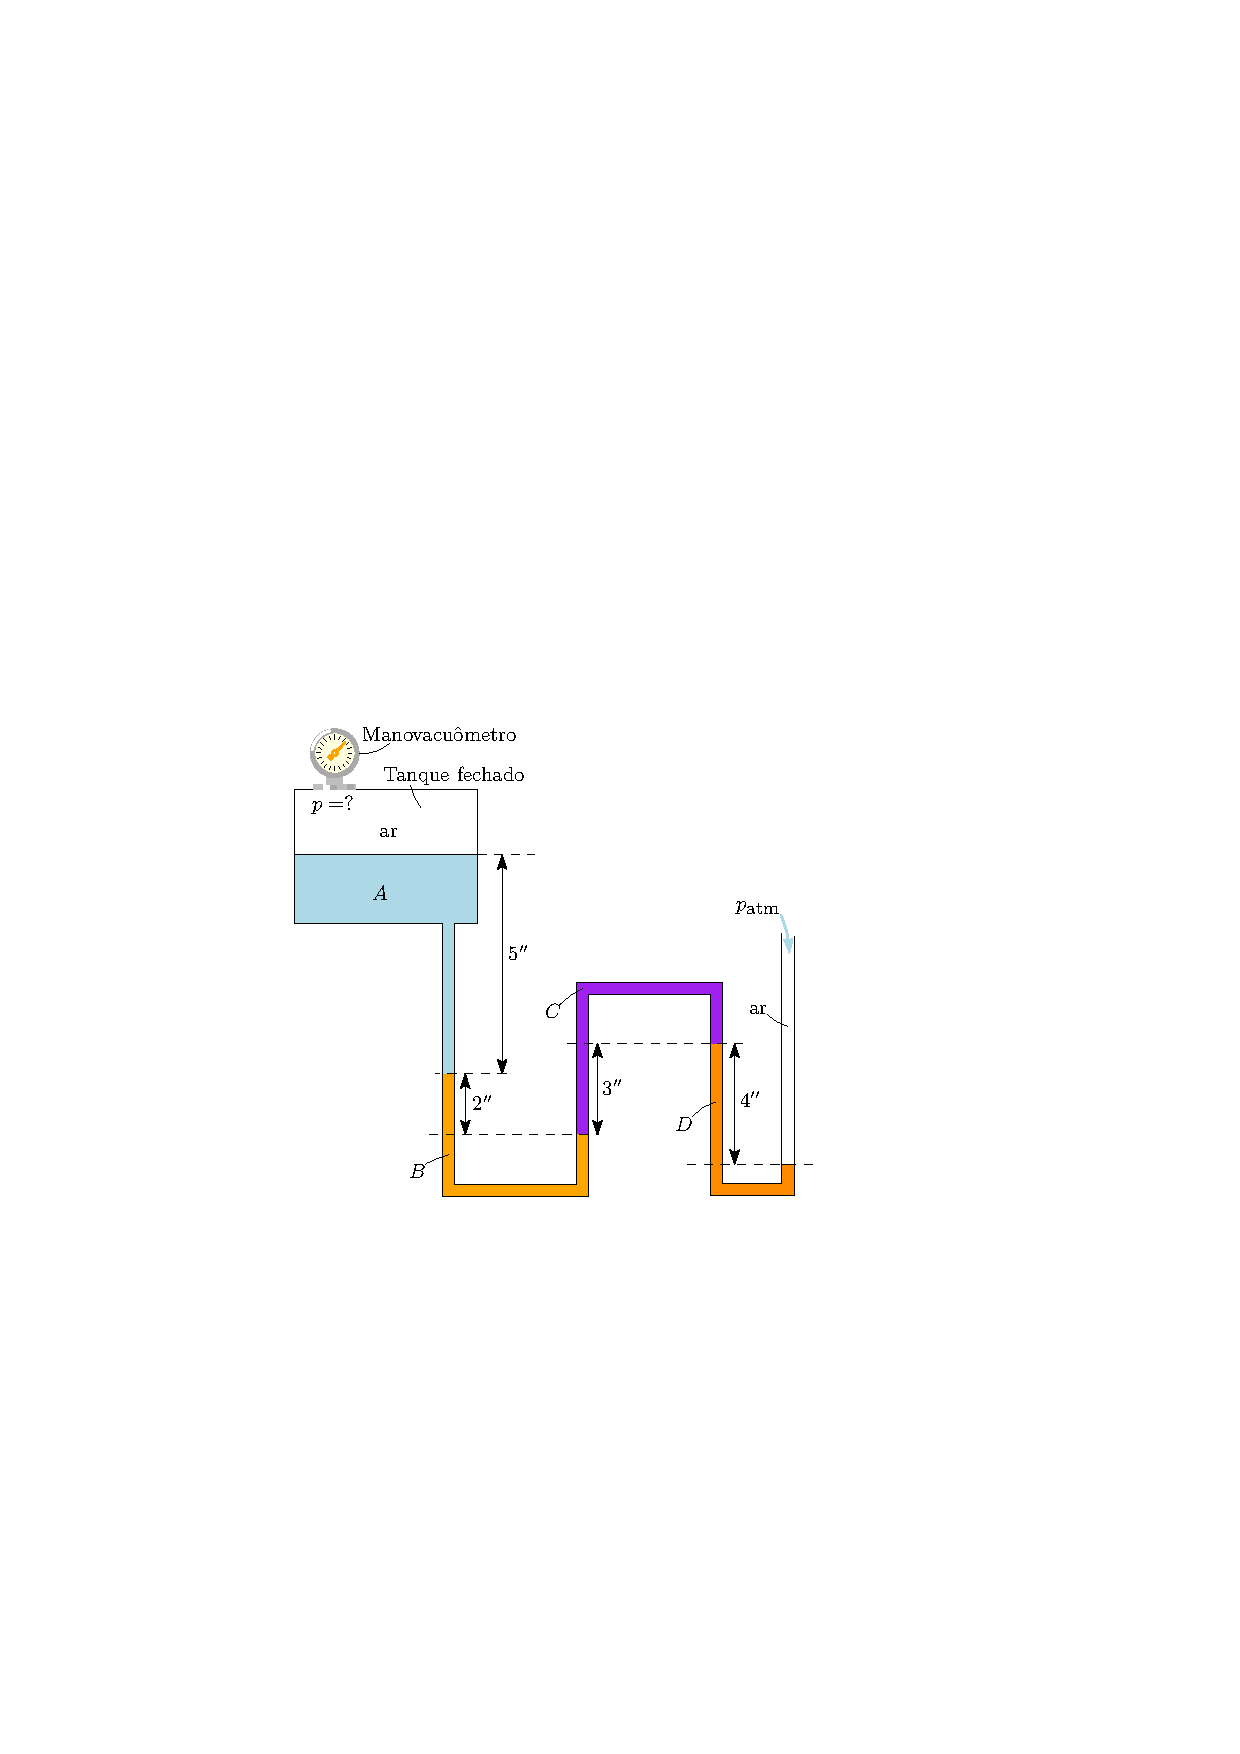
\includegraphics[width=.7\linewidth]{assets/images/ex5}
	\end{center}
	Com base nas cotas tracejadas feitas nos tubos ao realizar a análise percorrendo o sistema partindo do tubo com a extremidade sujeita à pressão atmosférica e tendo como referência os pontos numerados de 1 a 8
	\begin{center}
		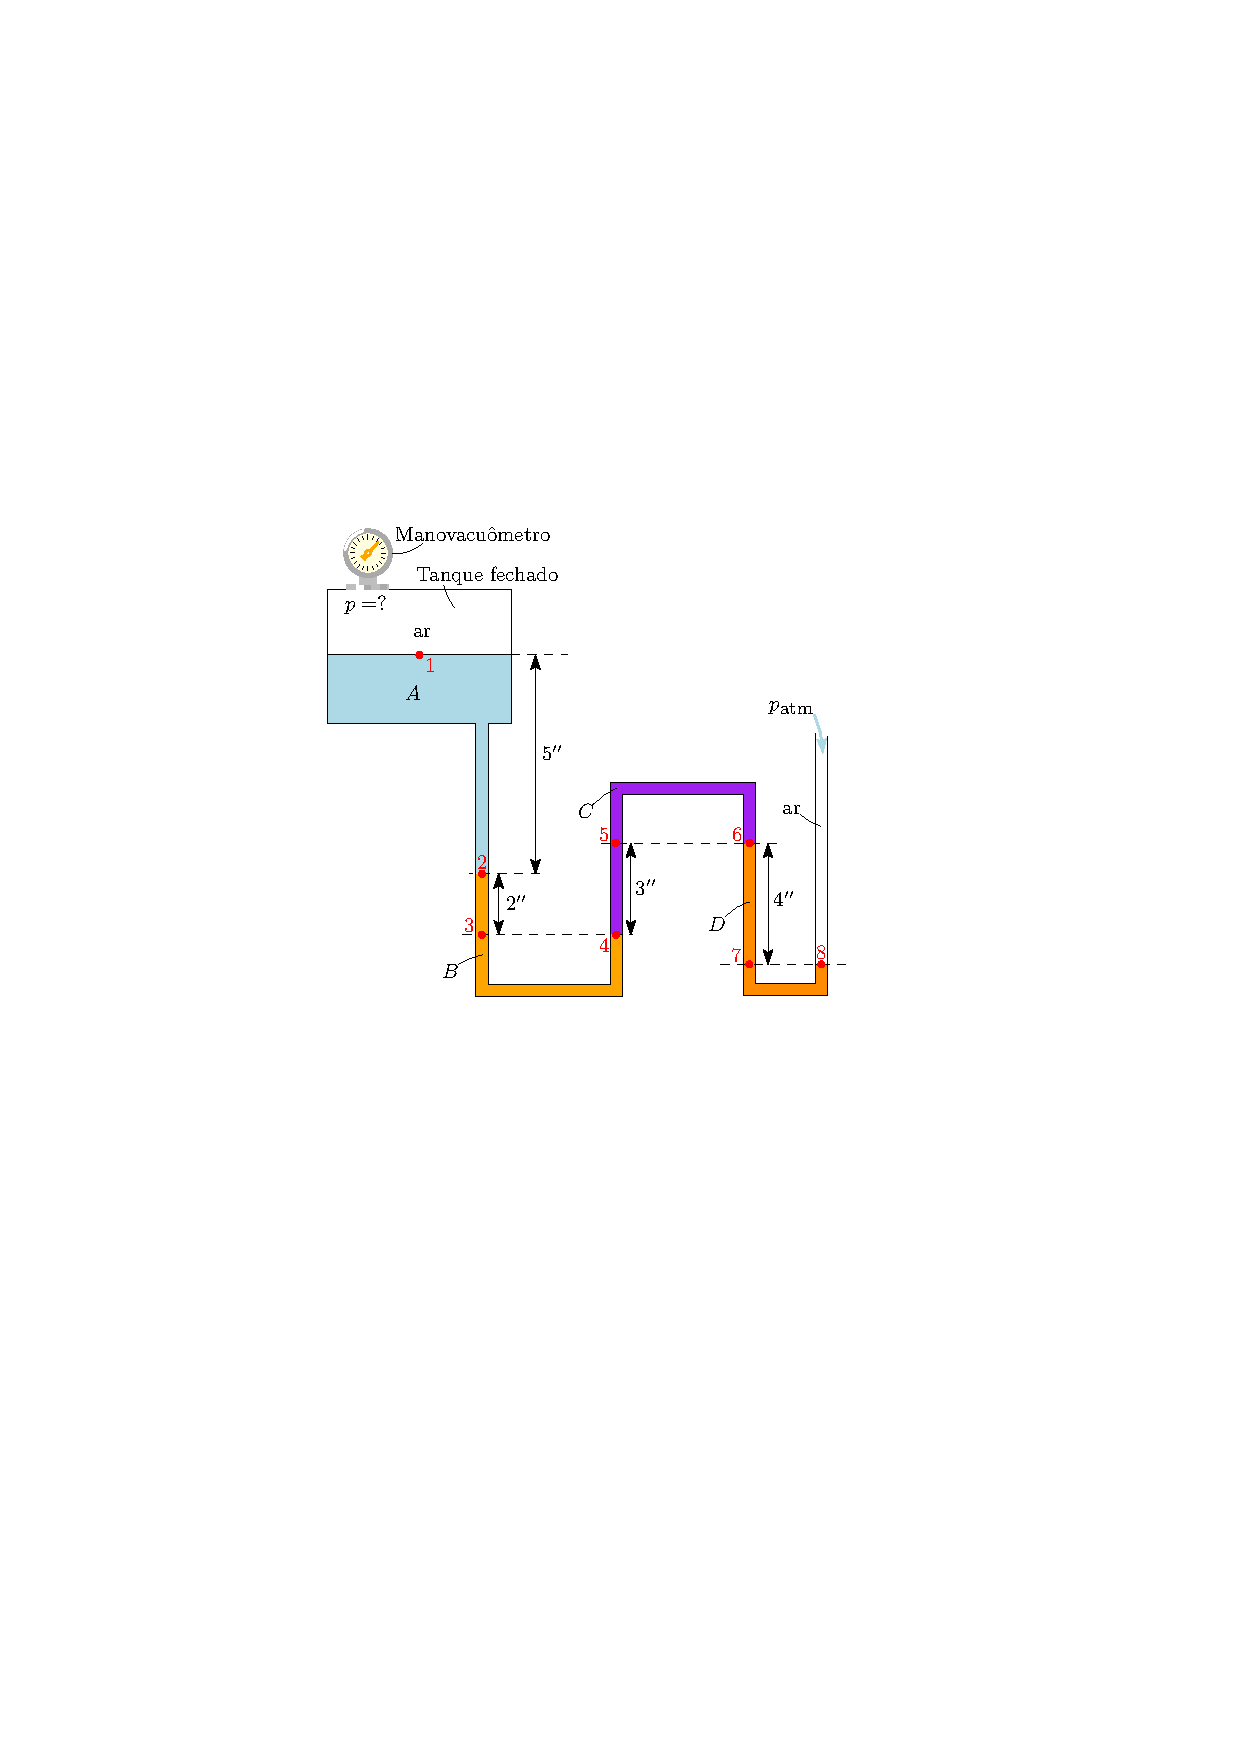
\includegraphics[width=.7\linewidth]{assets/images/pontos_5}
	\end{center}
	\begin{equation}
		p_{8}=p_{7}=p_{\textrm{atm}}=0
	\end{equation}
	\begin{eqnarray}
		\cancel{p_{7}}-p_{6}&=&\gamma_{D}\cdot 4''\\
		p_{6}&=&p_{5}=-\gamma_{D}\cdot 4''
	\end{eqnarray}
	\begin{eqnarray}
		p_{4}-p_{5}&=&\gamma_{C}\cdot 3''\\
		p_{4}&=&\gamma_{C}\cdot 3''-\gamma_{D}\cdot 4''
	\end{eqnarray}
	Como $p_{4}=p_{3}$
	\begin{eqnarray}
		p_{3}-p_{2}&=&\gamma_{B}\cdot 2''\\
		p_{2}&=&\gamma_{C}\cdot 3''-\gamma_{D}\cdot 4'-\gamma_{B}\cdot 2''
	\end{eqnarray}
	\begin{eqnarray}
		p_{2}-p_{1}&=&\gamma_{A}\cdot 5''\\
		p_{1}&=&\gamma_{C}\cdot 3''-\gamma_{D}\cdot 4''-\gamma_{B}\cdot 2''-\gamma_{A}\cdot 5''
	\end{eqnarray}
	\begin{eqnarray}
		p_{1}&=&p\\
		&=&(\rho_{C}\cdot 3-\rho_{D}\cdot 4-\rho_{B}\cdot 2-\rho_{A}\cdot 5)\cdot g\cdot\xi\\
		&=&(1300\cdot 3-6900\cdot 4-5400\cdot 2-2300\cdot 5)\cdot 9.81\cdot 0.0254\\
		&=&\SI{-11462.004}{\pascal}\\
		&=&-11.462004\cdot 0.01\\
		&=&\SI{-114.6}{\milli\bar}
	\end{eqnarray}
\end{document}